\chapter{Design and Experiments}
Summary of the experiment results and their details laid out in this section.
Neural network experiment logs are published online for more detailed examination, they are accessible by the url provided in the corresponding footnotes of this section.

\section{Training Specifications}
Training for traditional machine learning used in this project is fallows two step approach.
At the first part hyper-parameters for the model is selected by cross validation score then in the second part model is trained on entire dataset with the selected hyper-parameters.
Final model then evaluated on the test set.

There are many artificial neural networks used in both in benchmarking and the model selection.
Weights of the networks initialized by random except for the transfer learning models.
Model used in the transfer learning experiments initialized with the weighs pre-trained on imagenet~\cite{imagenet} dataset.
Each architecture is trained end-to-end using Adam~\cite{adam} optimizer with the standard parameters ($\beta_1 = 0.9$ \& $\beta_2 = 0.999$).
I used batch size of 64 for the training, and initial learning rate of 0.001 that decayed by the factor of 10 every time validation loss stagnates after an epoch.
Each image in the dataset is is downscaled to $224 \times 224$ size and normalized values to between zero to one.
Data augmentation is applied to minority class in the dataset to create a balanced dataset as explained in section \ref{sec:dataprocessing}.
Random cropping, changing saturation and horizontal flipping are set of augmentations chosen to create a balanced dataset.


\section{Benchmark Experiments}

\subsection{Random Forest Classifier and SVM}
Cross validation results of the random forest classifier found the fallowing hyper-parameters achieves the best performance:

\begin{itemize}
    \item Number of trees: 500
    \item Information gain criteria: Gini
    \item Number of max features: Square root
    \item Bootstrap: allowed
\end{itemize}

Cross validation for the support vector machine classifier runs suggested the fallowing hyper-parameters will achieve the best metrics:

\begin{itemize}
    \item Regularization parameter: 10
    \item Kernel: rbf
    \item Polynomial degree: 3
    \item Kernel coefficient $\gamma$: scale
    \item Tolerance: 0.001
\end{itemize}

Confusion matrix of these classifiers evaluated on test data generated fallowing results.

\begin{figure}[H]%
    \centering
    \subfloat[Random forest]{{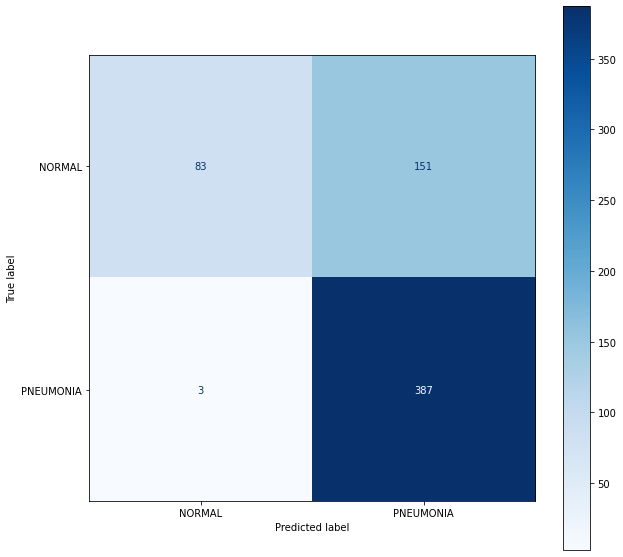
\includegraphics[width=.4\textwidth]{img/rf-confusion-matrix.png} }}%
    \qquad
    \subfloat[SVC]{{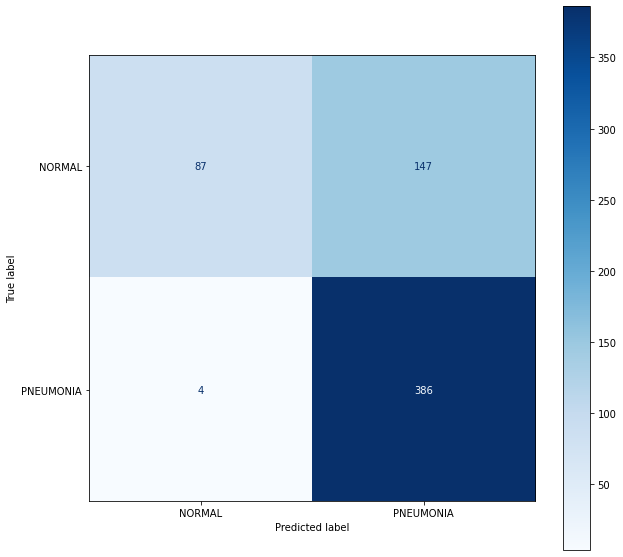
\includegraphics[width=.4\textwidth]{img/svm-confusion-matrix.png} }}%
    \caption{Confusion matrix of the classifiers.}%
    \label{fig:cmatrix}%
\end{figure}

It is clear from the amount of wrongly classified healthy patience X-ray, both of the models suffer from the imbalance effect.
This effect is slightly more dominant in the random forest classifier than the SVC, albeit performance of both model are similar.

\begin{table}[H]
    \centering
    \begin{tabular}{||c c c c c||} 
    \hline
    Classifier & Accuracy & Precision & Recall & f1\\ [0.5ex] 
    \hline\hline
    Random Forest & 0.7532 & 0.3547 & 0.9650 & 0.5187\\ 
    \hline
    SVC & 0.7580 & 0.3718 & 0.9560 & 0.5354\\
    \hline
    \end{tabular}
    \caption{Performance metrics for traditional machine learning algorithms.}
    \label{table:mlmetrics}
\end{table}



\subsection{AlexNet}
During the experiments for AlexNet and LeNet5 effect of the balanced~\footnote{AlexNet Balanced: https://tensorboard.dev/experiment/7b6W0tdHQQ2RINGt6cYbrA/} dataset is also compared to base~\footnote{AlexNet Base: https://tensorboard.dev/experiment/PaBawCErSqG6zIef7JPq8g/} dataset to mesure the effectiveness of the data augmentation.
Figures used in AlexNet and LeNet5 annotated with balanced training/val to reflect that balanced dataset is created with the data augmentation.
Base training/val is used to refer base image data is used without and data augmentation.
Results from AlexNet was average but given the loss values did not declined in the validation dataset suggest that ALexNet slightly over-fitted the data.

\begin{figure}[H]
    \centering
    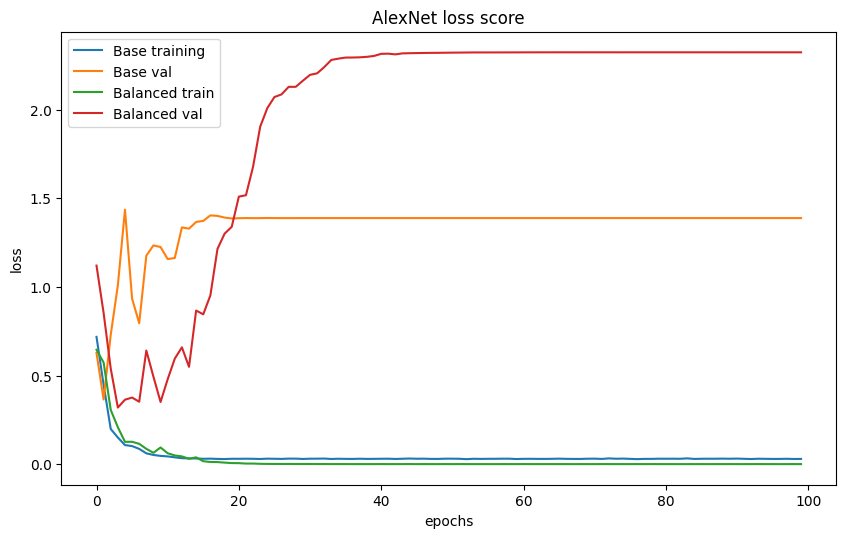
\includegraphics[width=.9\textwidth]{img/alexnetloss.png}
    \caption{}
    \label{fig:alexloss}
\end{figure}

Another important point is that converge was very quick for this particular dataset. 
It is clearly visible in the charts that model converge in around first 30 epochs and remained unchanged for the rest of the training.

\begin{figure}[H]
    \centering
    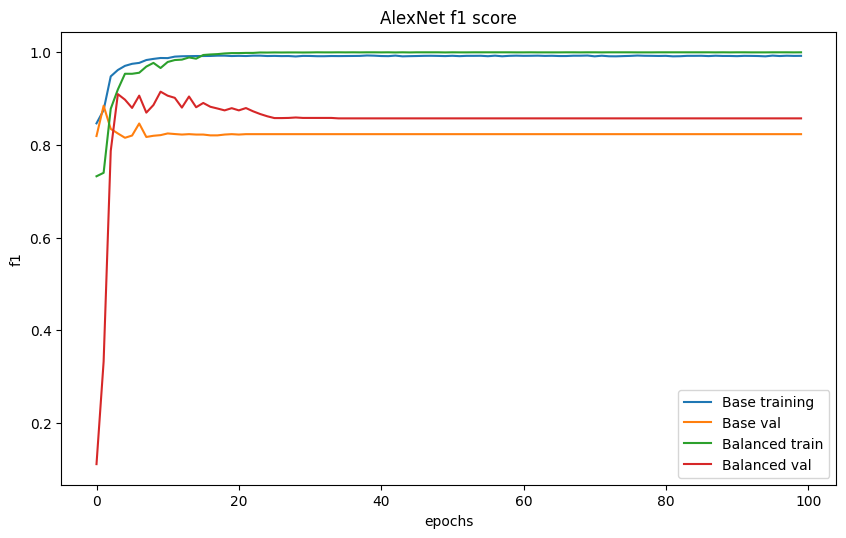
\includegraphics[width=.9\textwidth]{img/alexnetf1.png}
    \caption{}
    \label{fig:alexf1}
\end{figure}


\subsection{LeNet-5}
I was not able to train the LeNet5 model with the original model specification that utilize hyperbolic tangent function (tanh).
This was partially expected as tanh activation function is not able to pass the gradient flow very well when the initialization is not favorable.
This effect is mentioned in the section \ref{sec:gradients} and as such I have replaced the activation function with the ReLu activation function for my implementation.
Similar to AlexNet, LeNet5 also displayed possible sign of over-fitting when loss did not declined on the validation dataset.

\begin{figure}[H]
    \centering
    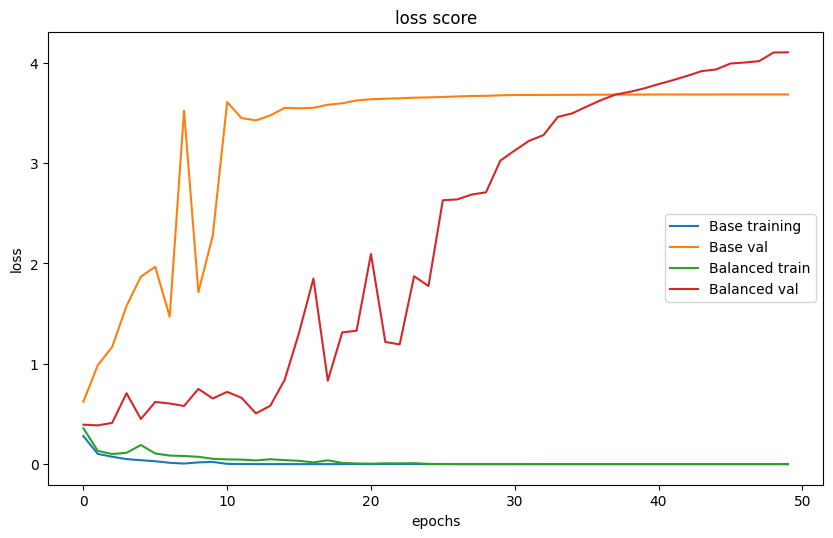
\includegraphics[width=.8\textwidth]{img/lenetloss.png}
    \caption{LeNet5 loss metrics}
    \label{fig:lenetloss}
\end{figure}

\begin{figure}[H]
    \centering
    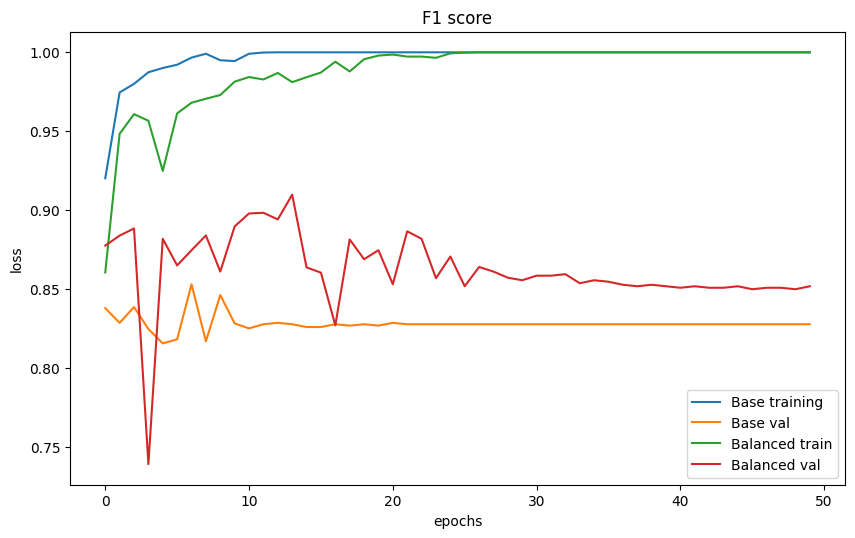
\includegraphics[width=.8\textwidth]{img/lenetf1.png}
    \caption{LeNet5 f1 metrics}
    \label{fig:lenetloss}
\end{figure}



\subsection{VGGNet}
Performance of this model~\footnote{VGGNet Base: https://tensorboard.dev/experiment/IbsPnocxSMKqNjmdJ3CdpA/}~\footnote{VGG Balanced: https://tensorboard.dev/experiment/ABd8GrKdSXyzHgNPDngeEw/} is the worst among all of the model I tried.
Disappointing performance didn't change with the different random initialization.
However, training and validation loss suggested a good training, accuracy metric was below random guess.

\begin{figure}[H]
    \centering
    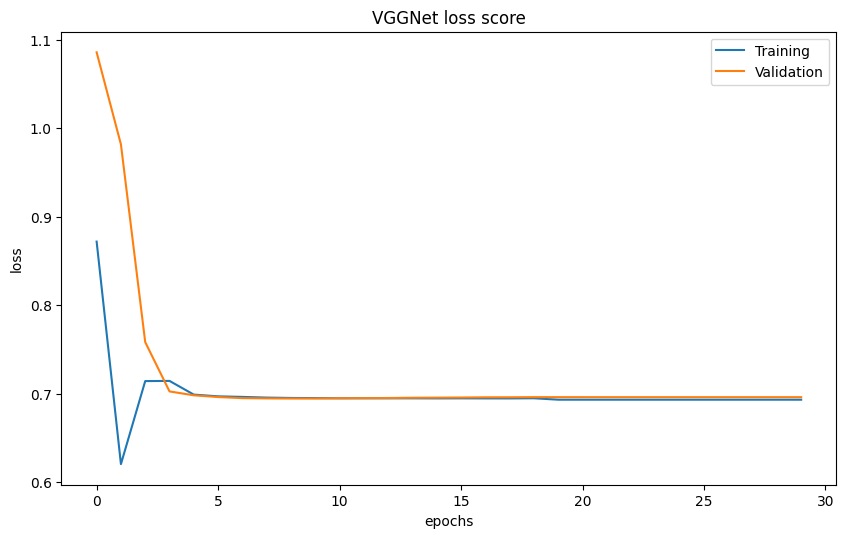
\includegraphics[width=.8\textwidth]{img/vggnetloss.png}
    \caption{}
    \label{fig:vggloss}
\end{figure}

\begin{figure}[H]
    \centering
    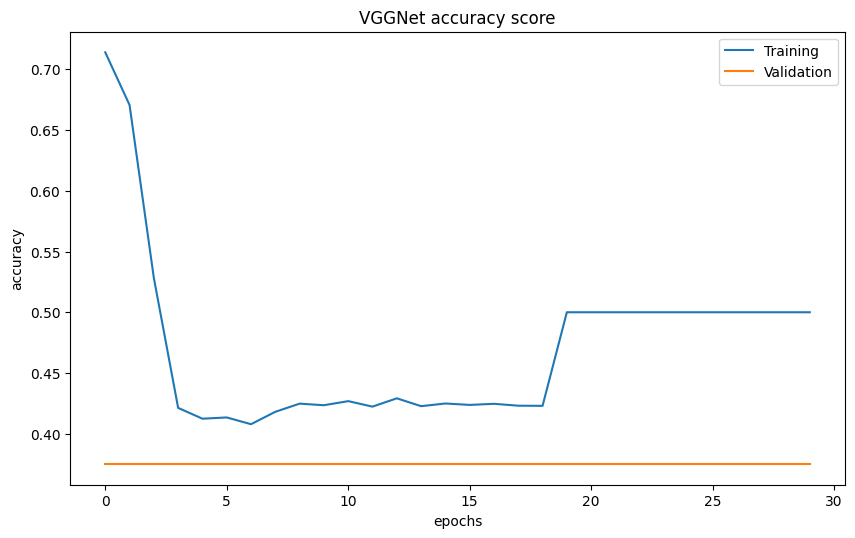
\includegraphics[width=.8\textwidth]{img/vggnetaccuracy.png}
    \caption{}
    \label{fig:vggacc}
\end{figure}

% vggnet https://tensorboard.dev/experiment/IbsPnocxSMKqNjmdJ3CdpA/
% vgg balanced https://tensorboard.dev/experiment/ABd8GrKdSXyzHgNPDngeEw/

\section{Transfer Learning}
I was very skeptical when adopting transfer learning to pneumonia detection because of the fundamental difference in the type of images in the imagenet compare to project dataset.
In this implementation weights in the convolutional part of the model initialized with the pre-trained VGGNet model from imagenet dataset.
Convolution layer weights in this network is kept frozen during the training and allowed only fully connected layers at the end of the model to be trained.
To my surprise this approach worked considerably well. Achieving $\approx 77 \%$ in accuracy and $\approx 87 \%$ f1 on validation data. 

\begin{figure}[H]
    \centering
    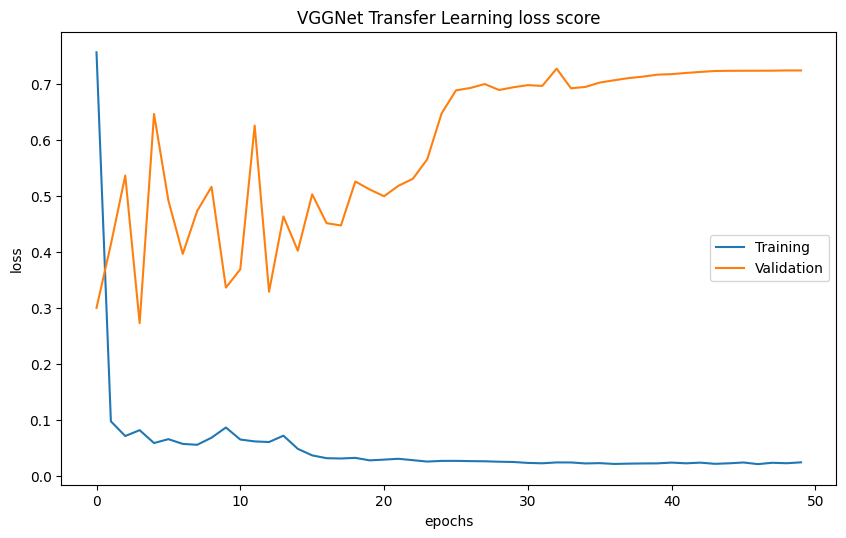
\includegraphics[width=.8\textwidth]{img/vggnettfloss.png}
    \caption{}
    \label{fig:vggtfloss}
\end{figure}

\begin{figure}[H]
    \centering
    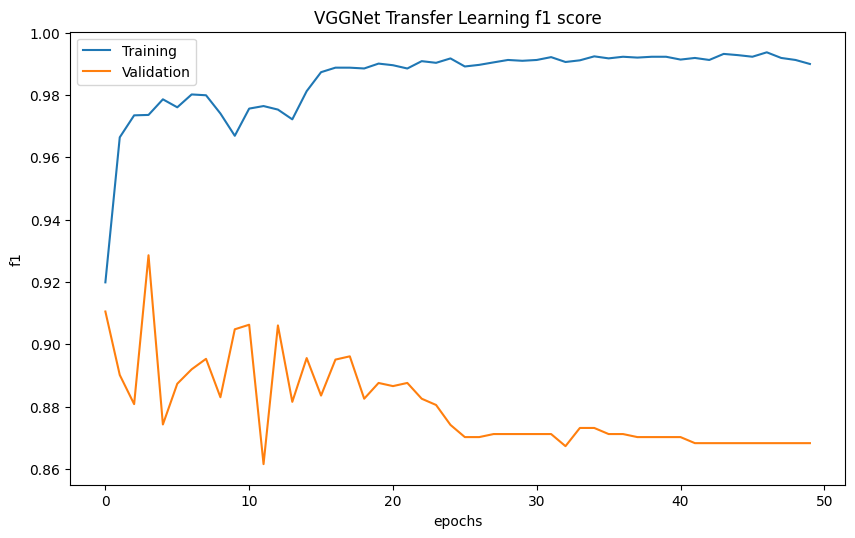
\includegraphics[width=.8\textwidth]{img/vggnettff1.png}
    \caption{}
    \label{fig:vggtff1}
\end{figure}

% \begin{figure}[H]
%     \centering
%     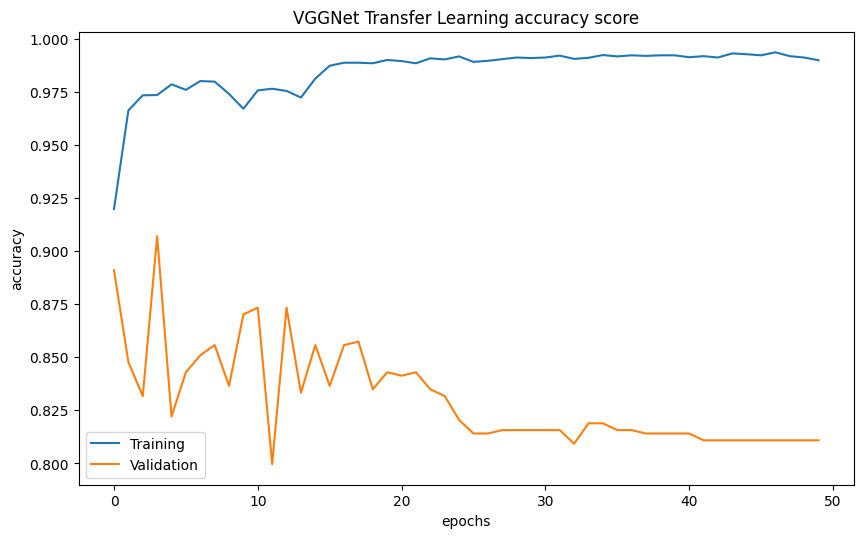
\includegraphics[width=.8\textwidth]{img/vggnettfaccuracy.png}
%     \caption{}
%     \label{fig:vggtfacc}
% \end{figure}
% vgg https://tensorboard.dev/experiment/VxxyXkn6TaSMrgKnSP1low/
% vgg-balanced https://tensorboard.dev/experiment/c1zSx6N0QviARqCVIq3QMw/

\section{Custom Neural Network Architecture}
After experimenting with randomly choose number of layers best combination I discovered is an architecture with ten convolution layers fallowed by batch normalization and max-pooling layer. 
In final experiments showed using two convolutional layer fallowed by batch normalization layer and max-pooling layer like a convolutional block is an optimal choice for this architecture.

\begin{figure}[H]
    \centering
    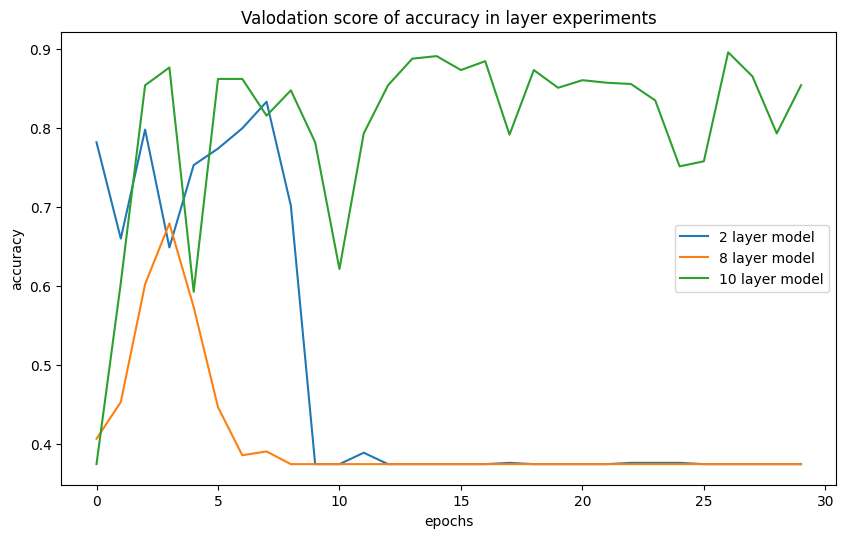
\includegraphics[width=\textwidth]{img/layerexpaccuracy.png}
    \caption{}
    \label{fig:layerexpacc}
\end{figure}

Immediately after this experiments same number of layers are maintain to determine the performance of the type of the convolution layer on the dataset.
For the same number of layer I replaced the convolutional layers with the depthwise separable convolutional layers.
Depthwise separable convolutional layers works by performing a depthwise convolution first then mixing that with the pointwise convolution.
Result shows that convolutional layers perform better than depthwise convolutional layers whit the same layer numbers and other convolution properties set equally.

\begin{figure}[H]
    \centering
    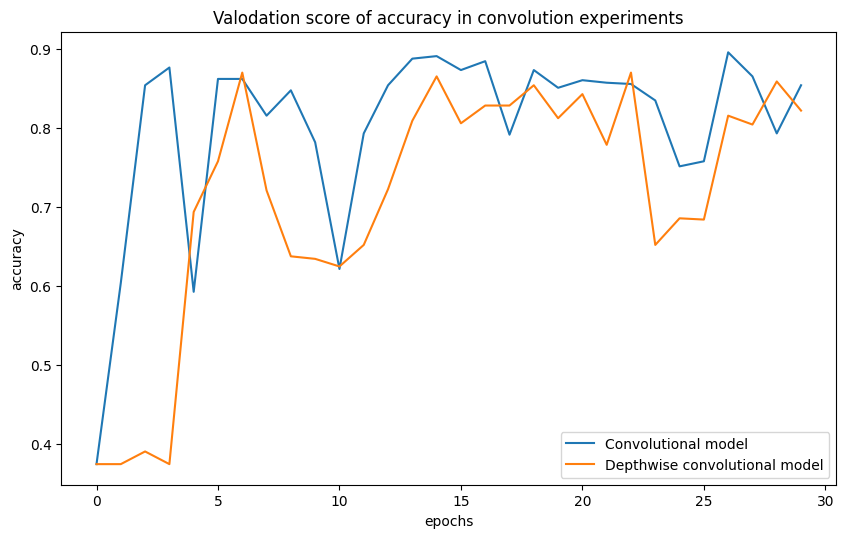
\includegraphics[width=.8\textwidth]{img/deptoconvexpaccuracy.png}
    \caption{}
    \label{fig:depttoconvacc}
\end{figure}

Lastly, I have started experiments to observe the effect of regularization at the fully connected layers.
Varying levels of dropout rate applied to dense layers to fine-tune the regularization level that best suits this architecture. Results shows that best level of dropout rate as 30\%, albeit dropout rates in the dense layers effect change very little the performance scores of the model.

\section{Interpreting Model Decisions}

% base (https://tensorboard.dev/experiment/p2mkNoLORACZlCXL2UQRbg)
% augmented (https://tensorboard.dev/experiment/dmQIbMeJQtqF70MhQQqySA)